\documentclass[aspectratio=169,11pt]{beamer}
% Shared preamble for the CogLean decks.
% Build the slides alone, or with speaker notes (see the Makefile):
%   pdflatex deck.tex                                   -> slides
%   pdflatex -jobname=deck-notes "\def\withnotes{}\input{deck.tex}"  -> slides + notes
\usetheme{default}
\usecolortheme{seahorse}
\setbeamertemplate{navigation symbols}{}
\setbeamertemplate{footline}[frame number]
\setbeamerfont{note page}{size=\small}
\ifdefined\withnotes
  \setbeameroption{show notes}
\fi
\usepackage[T1]{fontenc}
\usepackage{lmodern}
\usepackage{booktabs}
\usepackage{amsmath,amssymb}
\usepackage{tikz}
\usetikzlibrary{positioning,arrows.meta,shapes.misc}
\tikzset{
  box/.style={draw, rounded corners, align=center, minimum height=8mm, inner sep=4pt, fill=blue!6},
  arr/.style={-{Stealth[length=2mm]}, thick}
}
\newcommand{\code}[1]{\texttt{#1}}
\newcommand{\has}{\textbf{has}}
\newcommand{\lacks}{\textcolor{red!70!black}{lacks}}
\newcommand{\never}{\textcolor{red!70!black}{\textbf{never}}}
\newcommand{\canhold}{can hold}


\title{Multi-digit addition: one model from many}
\subtitle{Recognition, associations, problem solving, and memory, composed and proved}
\author{Jeff Shrager}
\date{October 2026}

\begin{document}

\begin{frame}
  \titlepage
\end{frame}
\note{
This talk is about the largest model in CogLean: three-digit addition, built by composing theories that were each formalized on their own. EPAM's discrimination nets recognize the problem. Siegler and Shrager's distributions of associations retrieve answers and single-digit facts. A problem solver, in the GPS and repair-theory tradition, works the columns. And the memory itself is a parameter, so ACT-R's declarative memory can be swapped in. I'll describe each component, how they compose, and what is proved about the whole that none of the parts says alone.
}

\begin{frame}{The task, and what a model must explain}
  \begin{itemize}
    \item Children and adults solve problems like $150 + 100$ and $478 + 256$.
    \item Some problems are \emph{familiar}: the answer is retrieved. Others are worked out, column by column.
    \item Errors come in kinds:
    \begin{itemize}
      \item \textbf{confident errors}: a familiar-looking problem answered with a neighbour's sum, with no hesitation;
      \item \textbf{column errors}: a single-digit fact wrong in one column;
      \item \textbf{procedural bugs}: systematic errors from a procedure with a missing step (no carry).
    \end{itemize}
  \end{itemize}
\end{frame}
\note{
The task is three-digit addition. Some problems are familiar and their answers are simply retrieved; others are worked out column by column. And the errors come in kinds that need different explanations. Confident errors: a problem that looks like a familiar one gets that problem's answer, with no hesitation. Column errors: a single-digit fact goes wrong in one column. And procedural bugs: systematic errors from a procedure missing a step, like never carrying. One model should produce all three, each for the right reason.
}

\begin{frame}{The architecture}
  \begin{center}
  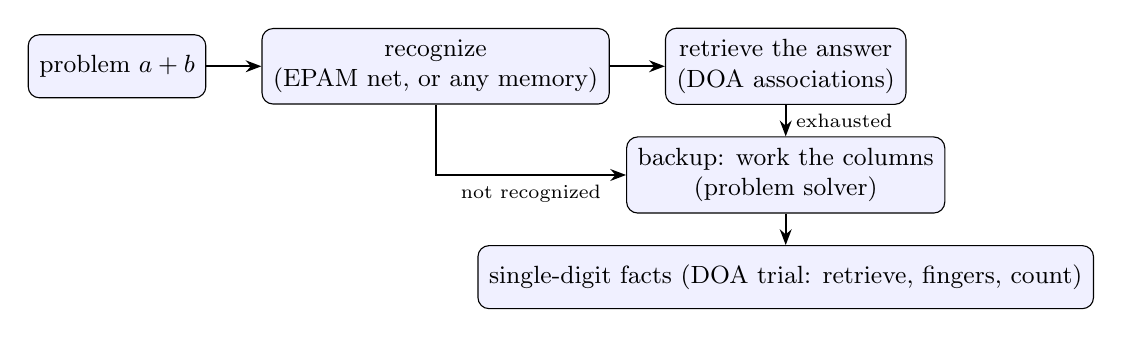
\begin{tikzpicture}[node distance=4mm and 7mm, every node/.style={font=\small}]
    \node[box] (p) {problem $a + b$};
    \node[box, right=of p] (r) {recognize\\(EPAM net, or any memory)};
    \node[box, right=of r] (w) {retrieve the answer\\(DOA associations)};
    \node[box, below=of w] (b) {backup: work the columns\\(problem solver)};
    \node[box, below=of b] (f) {single-digit facts (DOA trial: retrieve, fingers, count)};
    \draw[arr] (p) -- (r); \draw[arr] (r) -- (w);
    \draw[arr] (w) -- node[right, font=\scriptsize] {exhausted} (b);
    \draw[arr] (r.south) |- node[below, pos=0.75, font=\scriptsize] {not recognized} (b.west);
    \draw[arr] (b) -- (f);
  \end{tikzpicture}
  \end{center}
  Every arrow is a composition of probability distributions; every box is a theory formalized on its own, with its own theorems.
\end{frame}
\note{
Here's the architecture. A problem is first recognized, by an EPAM discrimination net or, since memory is a parameter, by any memory. If it's recognized, the answer is retrieved from that problem's distribution of associations. If retrieval is exhausted, or nothing is recognized, the backup takes over and works the columns, and that backup is now a problem solver. Each column needs a single-digit fact, which comes from a full distributions-of-associations trial: retrieve, or put up fingers, or count. Every arrow is a composition of probability distributions, and every box is a theory that was formalized and proved on its own first.
}

\begin{frame}{Component 1: recognition (EPAM)}
  \begin{itemize}
    \item A \textbf{discrimination net} tests features of the problem's code, and sorts it to a stored image.
    \item Learning adds a test only where two codes are confused.
    \item A net that has never needed to tell two problems apart can't: $150 + 100$ is sorted to $100 + 100$ when the net tests only the digit where the familiar problems differ.
  \end{itemize}
  \medskip
  Proved for every net: recognition depends only on the features tested; a confusion agrees on every tested feature; learning a problem never disturbs another.
\end{frame}
\note{
The first component is EPAM's discrimination net. It tests features of the problem's code and sorts the problem to a stored image. Learning adds a test only where two codes are confused, so a net that has never needed to tell two problems apart can't. In our worked case, the net learned one hundred plus one hundred and one hundred plus two hundred, so it tests only the digit where they differ, and one hundred fifty plus one hundred is sorted to one hundred plus one hundred. The general theorems hold for every net: recognition depends only on tested features, a confusion agrees on all of them, and learning never disturbs other problems.
}

\begin{frame}{Component 2: distributions of associations (Siegler \& Shrager 1984)}
  \begin{itemize}
    \item Each problem has associations of varying strength to possible answers.
    \item Retrieval samples an answer in proportion to strength; it is stated if above a \textbf{confidence criterion}; up to a search length.
    \item If nothing is stated: backup strategies (fingers, counting fingers).
    \item Used twice here: for \textbf{whole problems} (once recognized) and for \textbf{single-digit facts} in each column.
  \end{itemize}
  \medskip
  Proved: retrieval is used with probability $1 - (1-R)^n$; the error share on retrieval trials is the wrong answers' share above the criterion; strengthening the correct answer never raises errors.
\end{frame}
\note{
The second component is the distributions-of-associations model that Bob Siegler and I proposed in 1984. Each problem has associations of different strengths to possible answers. Retrieval samples an answer in proportion to strength, states it if it's above a confidence criterion, and tries up to a search length; if nothing is stated, the child falls back on fingers or counting. In the combined model it's used twice: for whole problems once they're recognized, and for the single-digit fact in each column. Its own theorems hold throughout, for instance that strengthening the correct answer never raises the error rate.
}

\begin{frame}{Component 3: the column backup as problem solving}
  \begin{itemize}
    \item A problem space: add a column (its fact from a DOA trial), write, write and carry, finish.
    \item \textbf{The bridge}: the solver answers exactly as the old fixed column procedure did, for every problem and every fact process.
    \item \textbf{Means-ends analysis} (GPS) works units first, though its goal names no order.
    \item \textbf{Repair theory} (Brown \& VanLehn 1980): delete the carry rule, and a column sum of 10 or more is an impasse; its repairs are bugs (no carry: $15 + 17 = 22$).
  \end{itemize}
\end{frame}
\note{
The third component is new: the column backup as problem solving. Its operators are adding a column, with the fact from a distributions-of-associations trial, writing, writing and carrying, and finishing. A bridge theorem shows it answers exactly as the old fixed procedure did, for every problem, so everything proved before carries over. Means-ends analysis discovers the units-first order on its own. And with the carry rule deleted, as repair theory does, a column sum of ten or more is an impasse, and its repairs are bugs: fifteen plus seventeen becomes twenty-two.
}

\begin{frame}{Component 4: memory as a parameter}
  \begin{itemize}
    \item Recognition is any \textbf{retriever}: study, then retrieve a distribution over stored items.
    \item EPAM's net is one; ACT-R's declarative memory (activation, partial matching) is another.
    \item Three \textbf{laws} of memory, determinacy, certainty and stability, are enough for confident errors; EPAM's net has all three, ACT-R has none.
  \end{itemize}
  \bigskip
  So which errors a learner makes depends on which memory they have, and the laws say why.
\end{frame}
\note{
The fourth component is that memory is a parameter. Recognition is stated for any retriever, anything you can study items into and retrieve from. EPAM's net is one, and ACT-R's declarative memory, with activation and partial matching, is another. Three laws of memory, determinacy, certainty and stability, are enough to guarantee confident errors. EPAM's net has all three; ACT-R has none of them. So the kind of errors a learner makes depends on the kind of memory they have, and the laws say exactly why.
}

\begin{frame}{How they compose}
  A trial on problem $x$:
  \[
    \text{trial}(x) = \text{recognize}(x) \;\gg\!\!=\; \big(\text{retrieve the recognized problem's answer} \;\text{else}\; \text{backup}(x)\big)
  \]
  \[
    \text{backup}(x) = \text{add units} \gg\!\!= \text{write and carry} \gg\!\!= \text{add tens} \gg\!\!= \dots
  \]
  \[
    \text{add column} = \text{DOA trial on its digits} \gg\!\!= \text{record the sum}
  \]
  \begin{itemize}
    \item Each $\gg\!\!=$ is a two-stage draw: probabilities multiply along a path and add over paths.
    \item Composition is exact: no simulation anywhere; every number is a theorem.
    \item Because draws regroup (associativity), a theorem about a component holds inside the whole.
  \end{itemize}
\end{frame}
\note{
How do they compose? A trial is recognition, then either retrieval of the recognized problem's answer or the backup. The backup is a chain of problem-solving steps, and adding a column is itself a full distributions-of-associations trial on that column's digits. Each step is a two-stage draw: probabilities multiply along a path and add over paths. It's exact, with no simulation anywhere, and every number is a theorem. And because these draws regroup freely, a theorem proved about a component holds where that component sits inside the whole.
}

\begin{frame}{What the whole predicts}
  \small
  \begin{tabular}{p{0.38\linewidth}p{0.55\linewidth}}
    \toprule
    Prediction & From\\
    \midrule
    Confident errors: every retrieval of a confused problem is wrong, with no extra backup & recognition (EPAM laws) + sharp associations (DOA)\\
    A column error is a single-digit error moved to its place & problem solver + DOA facts\\
    Carrying adds no error of its own & problem solver (bridge)\\
    Procedural bugs only on carry problems & problem solver without the carry rule\\
    Learning removes a confusion without disturbing other problems & EPAM learning\\
    \bottomrule
  \end{tabular}
\end{frame}
\note{
Here's what the whole model predicts, and which parts each prediction comes from. Confident errors come from recognition, whose laws make the confusion certain, together with sharp associations. A column error is a single-digit error moved to its place, from the problem solver using distributions-of-associations facts. Carrying adds no error of its own, through the bridge. Procedural bugs appear only on carry problems, from the problem solver without its carry rule. And learning removes a confusion without disturbing other problems, from EPAM. Each row needs at least two theories; none is in any single one.
}

\begin{frame}{A worked case}
  \begin{center}
  \begin{tabular}{lcc}
    \toprule
    & EPAM & ACT-R\\
    \midrule
    $150+100$ answered 200 (the neighbour's sum) & $45/46$ & $225/529$\\
    $150+100$ answered correctly & $1/46$ & $383/1058$\\
    \midrule
    $15+17$, no carry rule, strict critics & \multicolumn{2}{c}{22, for every such learner}\\
    \bottomrule
  \end{tabular}
  \end{center}
  \begin{itemize}
    \item Values are exact, at settings chosen for illustration; the predictions above hold for every setting.
    \item With EPAM, the confusion is certain; with ACT-R, it is graded.
  \end{itemize}
\end{frame}
\note{
A worked case. With EPAM recognition and illustrative strengths, one hundred fifty plus one hundred is answered with its neighbour's sum, two hundred, forty-five times in forty-six, and correctly only once in forty-six. With ACT-R's memory instead, the confusion is graded, and correct answers are much more common. And with the problem solver missing its carry rule and strict critics, fifteen plus seventeen is twenty-two. These numbers are exact but come from chosen settings; the predictions on the previous slide hold for every setting.
}

\begin{frame}{Is the formalization faithful?}
  \begin{itemize}
    \item A prose specification, with no Lean in it, and preregistered predictions.
    \item A fresh AI agent, given only the prose, wrote a Python simulator.
    \item \textbf{No failures}: 243 outcome frequencies on 4 instances matched Lean's exact values; every applicable prediction passed.
    \item It also found five vacuous predictions and a gap in the formalization, since fixed or recorded.
  \end{itemize}
  \medskip
  The blind check predates the problem solver; by the bridge, its results carry over unchanged.
\end{frame}
\note{
Is the Lean model the model described in prose? We checked with a blind simulation. A prose specification with no Lean in it, predictions preregistered before any simulator existed, and a fresh AI agent that wrote a Python simulator from the prose alone. There were no failures: two hundred forty-three outcome frequencies matched Lean's exact values. It also found five vacuous predictions and a gap in the formalization. The check was run before the problem solver existed, but because of the bridge theorem, its results carry over unchanged.
}

\begin{frame}{What each component contributes}
  \footnotesize
  \begin{tabular}{p{0.2\linewidth}p{0.2\linewidth}p{0.5\linewidth}}
    \toprule
    Component & Source & Role in the whole\\
    \midrule
    Discrimination nets & EPAM (Feigenbaum; Simon) & which problems look alike; certain confusions\\
    Distributions of associations & Siegler \& Shrager 1984 & answers, confidence, backup choice; single-digit facts\\
    Problem solving & GPS; Brown \& VanLehn 1980 & the column procedure; its order; its bugs\\
    Retrievers and laws & ACT-R; CogLean & which memory gives which errors, and why\\
    \bottomrule
  \end{tabular}
  \bigskip

  \normalsize
  Each was formalized and proved on its own; the composition is proved too.
\end{frame}
\note{
To summarize the parts. Discrimination nets, from EPAM, say which problems look alike and make confusions certain. Distributions of associations, from Siegler and Shrager, give answers, confidence and the choice of backup, and also the single-digit facts. Problem solving, from GPS and repair theory, gives the column procedure, its order and its bugs. And retrievers with laws of memory say which memory gives which errors, and why. Each was formalized and proved on its own, and the composition is proved too.
}

\begin{frame}{Limits, and next}
  \begin{itemize}
    \item Worked cases use chosen settings; priors should come from experience, as Siegler \& Shrager's did from counting (open issue).
    \item ``Multi-digit'' is three-digit.
    \item \textbf{Chunking} would close the loop: a fact found by counting at a retrieval impasse becomes an association, DOA's learning rule as problem-solving learning.
    \item Subtraction, borrowing, and repair theory's own bug data.
  \end{itemize}
\end{frame}
\note{
Limits. The worked cases use settings chosen for illustration; the prior associations should come from experience, as Siegler and Shrager's came from counting, and that's an open issue. Multi-digit here means three-digit. Next, chunking would close the loop between the parts: a fact found by counting when retrieval reaches an impasse becomes an association, which is the distributions-of-associations learning rule seen as problem-solving learning. And subtraction, with borrowing, where repair theory's bug data are.
}

\end{document}
